% Lecture Template for ME3023 -  Measurements in Mechanical Systems - Tennessee Technological University
% Spring 2020 - Summer 2020 - Fall 2020 - Spring 2021 - Summer 2021
% Tristan Hill, May 07, 2020 - June 12, 2020 - July 08, 2020 - Novemeber 02, 2020 - March 28, 2021 - May 25, 2021
% Module Name: To Err is Human
% Topic 1 - Accuracy and Error

\documentclass[fleqn]{beamer} % for presentation (has nav buttons at bottom)

%\usepackage{/home/thill/Documents/lectures/measurements_lectures/measurements_lectures}
%\usepackage{/home/thill/courses/measurements_lectures/measurements_lectures}
\usepackage{/home/tntech.edu/thill/courses/measurements_lectures/measurements_lectures}


\author{ME3023 - Measurements in Mechanical Systems} 

%\newcommand{\MNUM}{2\hspace{2mm}} % Module number
\newcommand{\TNUM}{1\hspace{2mm}} % Topic number 
\newcommand{\moduletitle}{To Err is Human}
\newcommand{\topictitle}{Accuracy and Error} 

\newcommand{\sectiontitleI}{Accuracy and Error}
\newcommand{\sectiontitleII}{Estimating Error}
\newcommand{\sectiontitleIII}{Uncertainty Interval}
\newcommand{\sectiontitleIV}{Activity with Data!}

% custom box
\newsavebox{\mybox}

\title{Lecture Module - \moduletitle}

\date{Mechanical Engineering\vspc Tennessee Technological University}

\begin{document}
	
	\lstset{language=MATLAB,basicstyle=\ttfamily\small,showstringspaces=false}
	
	\frame{\titlepage \center\begin{framed}\Large \textbf{Topic \TNUM - \topictitle}\end{framed} \vspace{5mm}}

% Section 0: Outline
\frame{

\large \textbf{Topic \TNUM - \topictitle} \vspace{3mm}\\

\begin{itemize}

	\item \hyperlink{sectionI}{\sectiontitleI} \vspc % Section I
	\item \hyperlink{sectionII}{\sectiontitleII} \vspc % Section II
	\item \hyperlink{sectionIII}{\sectiontitleIII} \vspc %Section III
	\item \hyperlink{sectionIV}{\sectiontitleIV} \vspc %Section IV

\end{itemize}

}

% Section 1
\section{\sectiontitleI}
	\begin{frame}[label=sectionI]
		\frametitle{\sectiontitleI}

		The exact value of a variable is called the \hspcu \hspc \hspcu. The value of the variables as indicated by a
		measurement system is called the \hspcu \hspc \hspcu. The \hspcu of a measurement refers to the
		closeness of agreement between the measured value and the true value. But the \hspcu \hspc \hspcu is rarely
		known \hspcu, and various influences, called \hspcu, have an effect on both of these values. So the
		concept of the \hspcu of a measurement is a \hspcu one. \vspcc

		\begin{framed}
			%\scalebox{1}{}$\hspace{10mm}{\RD error} = {\BL measured\hspace{1mm}value} - {\GR true\hspace{1mm}value} $}
		\end{framed}

		\vspace{0mm}
		{\tiny Text: Theory and Design of Mech. Meas.}
	\end{frame}

% Section 2
\section{\sectiontitleII}

	\begin{frame}[label=sectionII]
		\frametitle{\sectiontitleII}

		The \hspcu \hspc \hspcu can be estimated but cannot be known  \hspcu. In practice a \hspcu value is used in place of the true value. We will discuss this again the the {\it Calibration Module}.

		\begin{framed}%\scalebox{1}{$\hspace{20mm} {\PR accuracy} =  \frac{|{\RD error}|}{{\BR reference\hspace{1mm}value}}\times 100 $}
		\end{framed}

		An estimate of error based using this value is sometimes referred to as \hspcu \hspc \hspcu. \vspc
	\end{frame}

% Section 4
\section{\sectiontitleIV}

\begin{frame}[label=sectionIV]
	\frametitle{\sectiontitleIV}

	``The \hspcu is a numerical estimate of the possible range of the error in a measurement. In any
	measurement, the \hspcu is not known exactly since the true value is rarely known exactly. But based on
	available information, the operator might feel confident that the error is within certain bounds, a plus
	or minus range of the indicated reading. This is the assigned \hspcu.''\vspace{5mm}\\
	We will discuss this again the the {\it Uncertainty Module}.\vspace{10mm}\\

	{\tiny Text: Theory and Design of Mech. Meas.}
\end{frame}

% Section 4
\section{\sectiontitleIV}

	\begin{frame}[label=sectionIV]
		\frametitle{\sectiontitleIV}
		\scriptsize
		{\bf Experiment}: We are going to collect data with the sensor suite on our phones. \vspc
		
		\begin{multicols}{2}
		    Sensor:
		    \begin{itemize}
		    	\item GPS - \href{https://en.wikipedia.org/wiki/File:ConstellationGPS.gif}{concept graphic} 
		    	\item \href{https://www.garmin.com/en-US/aboutgps/}{info from manufacturer}  
		    \end{itemize}

		    Logger Apps:
			\begin{itemize}
				\item \href{https://www.tszheichoi.com/sensorlogger}{sensorlogger (Android) - Kelvin Choi} \vspc
				\item \href{https://apps.apple.com/us/app/sensor-logger/id1531582925}{Sensor Logger (OSX) -Choi Tsz Hei}
			\end{itemize}

			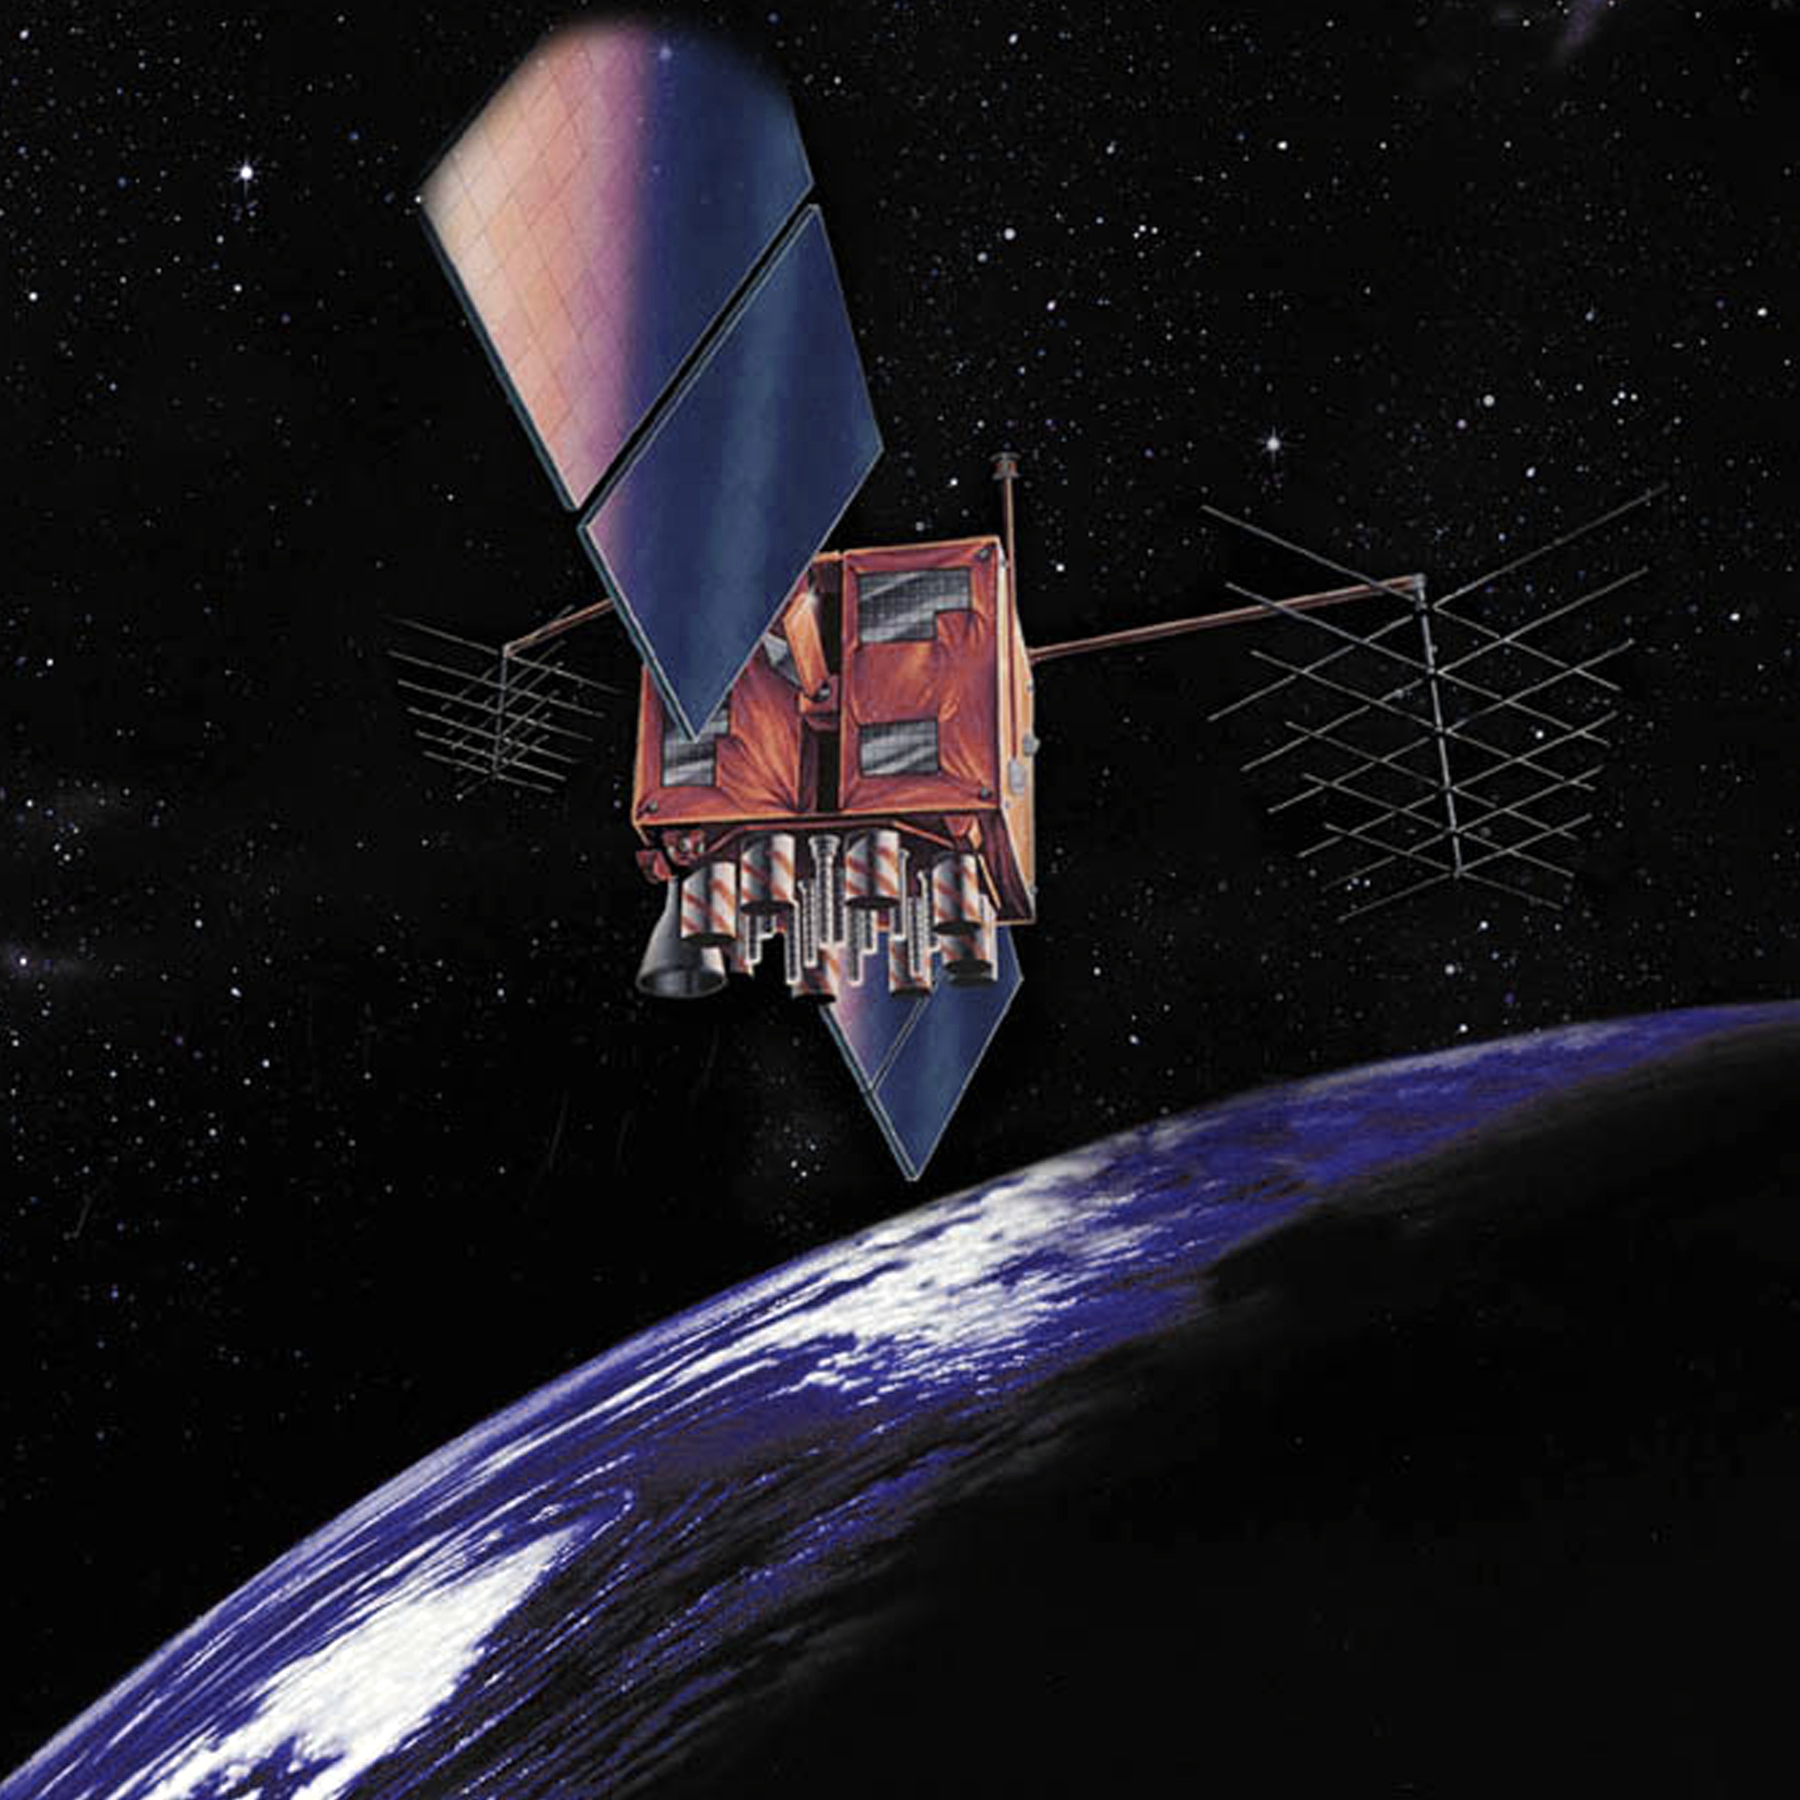
\includegraphics[scale=.075,angle=-90,origin=c]{GPS-IIR.jpeg}
			{\tiny Image:\href{https://en.wikipedia.org/wiki/Global_Positioning_System}{Wikipedia}}
		\end{multicols}	

	\end{frame}

	\begin{frame}[label=sectionIV]
		\frametitle{\sectiontitleIV}
		\scriptsize
		{\bf Part 1 - Informed Prediction}: Generate data you expect the GPS in your phone to report. Show the data points on the graph to the right.  \\
		
		\begin{multicols}{2}
			\setlength{\tabcolsep}{20pt}
			\renewcommand{\arraystretch}{1.4}
			\begin{tabular}{|c|c|c|} \hline
			$i$ & $lat_i$ & $lon_i$ \\\hline
			  1  & &              \\ \hline
			  2  & &              \\ \hline
			  3  & &              \\ \hline
			  4  & &              \\ \hline
			  5  & &              \\ \hline

			\end{tabular}

			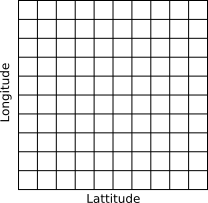
\includegraphics[scale=1]{lat_lon_grid.png}
			{\tiny Image: thill}
		\end{multicols}	

	\end{frame}

	\begin{frame}[label=sectionIV]
		\frametitle{\sectiontitleIV}
		\scriptsize
		{\bf Part 2 - Measurement}: Record GPS from your phone. Show the data points on the graph to the right. You can use export feature in Sensor Logger to report the data.  \\
		
		\begin{multicols}{2}

			\setlength{\tabcolsep}{20pt}
			\renewcommand{\arraystretch}{1.4}
			\begin{tabular}{|c|c|c|} \hline
			$i$ & $lat_i$ & $lon_i$ \\\hline
			  1  & &              \\ \hline
			  2  & &              \\ \hline
			  3  & &              \\ \hline
			  4  & &              \\ \hline
			  5  & &              \\ \hline
			  6  & &              \\ \hline
			  7  & &              \\ \hline
			  8  & &              \\ \hline
			  8  & &              \\ \hline		
			  9  & &              \\ \hline
             10  & &              \\ \hline
			\end{tabular}

			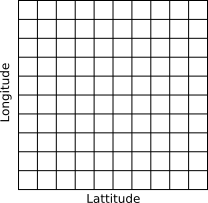
\includegraphics[scale=1]{lat_lon_grid.png}
			{\tiny Image: thill}
		\end{multicols}	

	\end{frame}

	\begin{frame}[label=sectionIV]
		\frametitle{\sectiontitleIV}
		\scriptsize
		{\bf Part 3 - Analysis/Results/Conclusions}: Compare and contrast the two sets of data. What conclusions can you make about your predictions or the sensor data?
		\begin{multicols}{2}

			\begin{itemize}
				\item Were the predictions reasonable? \\
				\item What type of error is present in the recorded data? \\
				\item What should be used as a reference for this data? \\ 
			\end{itemize}
			

			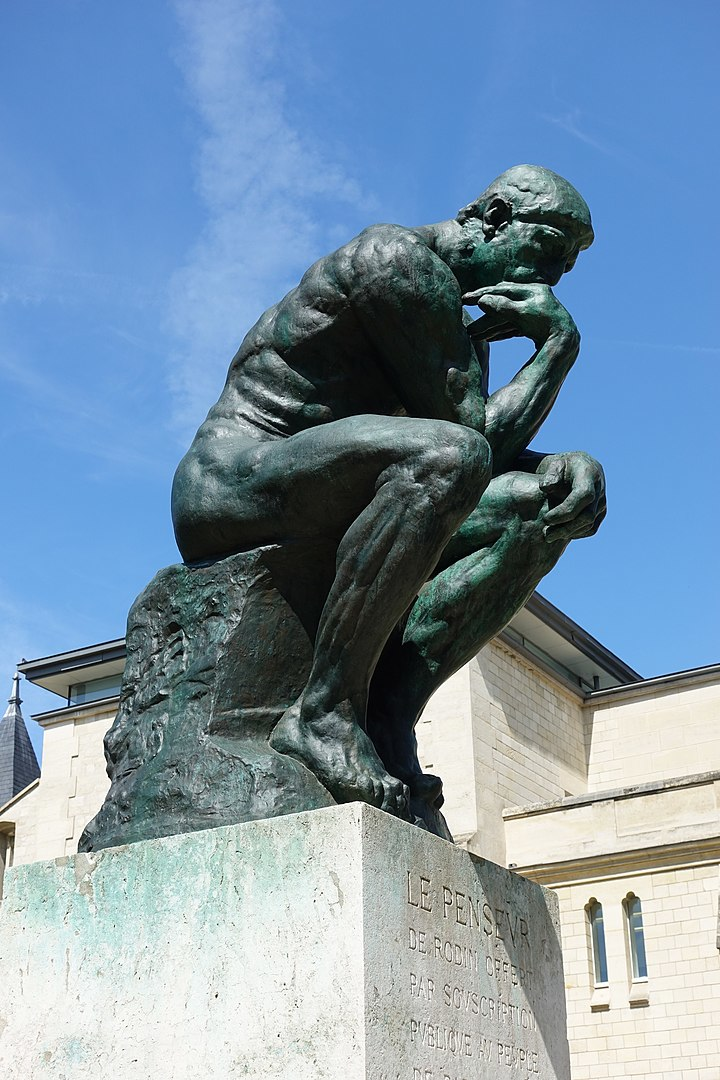
\includegraphics[scale=.071]{thinker_rodin.png}
			{\tiny Image: \href{https://en.wikipedia.org/wiki/The_Thinker}{wikipedia}}
			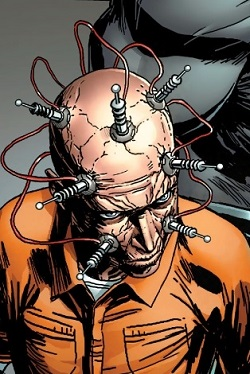
\includegraphics[scale=.15]{thinker_dc_comics.png}
			{\tiny Image: \href{https://en.wikipedia.org/wiki/Thinker_(DC_Comics)}{wikipedia}}
		\end{multicols}	

	\end{frame}

\end{document}





